% !TEX root = ../thesis.tex
\chapter{Implementation and Evaluation}
\label{ch:eval}
% **************************** Define Graphics Path **************************
\ifpdf
    \graphicspath{{Chapter5/Figs/Raster/}{Chapter5/Figs/PDF/}{Chapter5/Figs/}}
\else
    \graphicspath{{Chapter5/Figs/Vector/}{Chapter5/Figs/}}
\fi

\section{Introduction}
Chapter \ref{ch:approach} has proposed a real-time Crowd Monitoring Framework based on the Emotion Analysis of Social Media. This chapter describes our strategy to implement and evaluate the proposed framework using a case study. The case study analysed a past sporting event in which a stampede occurred and caused a number of injuries in the crowd. An experimental implementation of the framework was developed involving the data collection and the emotion extraction. Our evaluation was conducted by applying a series of statistical analyses on the emotion labelled dataset.

This chapter is structured as follows. Firstly, the case study is introduced. The next sections describe our implementation of the experiment, following by the evaluation. The chapter ends with the conclusion which will give a summarised view on the evaluation of our proposed framework.

\section{A Case Study using Historical Data}

The accuracy of the crowd type classification in our proposed framework relies on the Emotion Analysis and the Rule Based Reasoning. As presented in the Chapter \ref{ch:approach}, the Emotion Analysis extracts the emotion from the collected tweets about a gathering event and computes the emotion rates in the crowd. From the emotion rate, the level of an emotion can be determined using a threshold which will be discussed in this Chapter. Based on the levels of the four emotions, the Rule Based Reasoning finally identifies the correct crowd type or the group of crowd types using a set of defined rules.

In order to evaluate the accuracy of the approach, we conducted a case study using historical data because of the following reasons. Firstly, despite the large number of mass gathering events around the world, crowd accidents do not occur very often. For this reason, a case study with real-time data might require a considerably large number of experiments with incoming events until a potential detection is found. Nevertheless, when an accidents occurs, it is difficult to identify the exact crowd types that are present in an incident without an elaborate investigation.

Using historical data enables us to select an event in the past, where a crowd related accident eventually occurred and a known crowd type was identified. Our experiment will concentrate on the data retrieval and the comparison between the identified crowd types and the analysis results using our proposed Emotion - Crowd type Mapping Model and Rule Based Reasoning. Secondly, as our Bag-of-Words were constructed from an English corpus, experimenting with historical data also enables us to focus on the events in a English speaking country where a sufficient number of tweets in English can be collected for the Emotion Analysis.

One of the disadvantages of using historical data is that the performance of the framework regarding the real-time aspect cannot be tested. In order to evaluate whether the data collection technique can gather sufficient context data to support a real-time analysis or whether the result of the analysis is produced timely enough, further researches need to be done.

\subsection{Mayweather - Maidana Post Fight Stampede}

The first step of the experiment is to select a suitable mass gathering event that matches the criteria:
\begin{inparaenum}[i)]
\item the mass gathering took place in an English speaking country;
\item a crowd accident occurred and a known crowd type was identified;
\item the event was a recent event that preferably happened after 2012
\end{inparaenum}. The reason for the last criteria is that Twitter was created in 2006 and its traffic only started booming since 2012 \footnote{http://www.internetlivestats.com/twitter-statistics/}. Therefore, it is not possible to gather tweets about an event that happened too far in the past. For these reasons, we primarily looked for recent sporting events as these events tend to involve a large number of participants in highly arousing emotions. The boxing match in USA between Floyd Mayweather and Marcos Maidana on 3th May 2014 was selected. A stampede occurred after the fight \footnote{http://www.latimes.com/sports/sportsnow/la-sp-sn-mayweather-stampede-20140504-story.html}. 

The boxing match was held at the Grand Garden Arena of the MGM Grand Hotel in Las Vegas, USA with more than 16000 people attended \footnote{http://www.usatoday.com/story/sports/boxing/2014/05/04/floyd-mayweather-marcos-maidana-stampede/8700763/}. The match started at 6:00PM local time (UTC-7). The stampede occurred around 10:45PM during the post-fight news conference. The police received an emergency call at 10:45PM reporting a gunshot at the venue \footnote{http://lasvegassun.com/blogs/kats-report/2014/may/04/dozens-injuries-reported-after-stampede-mgm-grand-/}. According to the official statement, when the fans were leaving the arena, the stampede was triggered by a loud bang of a temporary wall falling over that was mistaken as a sound of a gunshot. It caused a massive panic and people started rushing to the exits. More than 50 people were trampled and crushed in the stampede and suffered from minor injuries. The situation got under control by 1:00 AM the next day. The layout of the arena was later criticized for having only two exits and the pathway was too narrow which has caused a bottleneck \footnote{http://sports.yahoo.com/news/bob-arum--stampede-after-mayweather-maidana-was--an-accident-ready-to-happen-004057893-boxing.html}.

This event appears to satisfy the criteria for our experiment. The next section will introduce our evaluation strategy using this case study.

\subsection{Evaluation Strategy}

As a stampede was confirmed to have occurred, the known crowd types for this event can be identified as escaping and dense/suffocating which belong to Group 4 motivated by fear in our classification in Chapter \ref{ch:approach}. The objective of the experiment was to verify whether our proposed approach can identify the correct crowd types or not.

A simple implementation of the crowd monitoring framework was performed. Firstly, the tweets regarding the event to construct our experimental dataset. Secondly, the Emotion Analysis was performed to extract the emotions from the tweets using the Bag-Of-Words approach and NRC Hashtag Emotion Lexicon \citep{mohammad2014using}. Because in the real-time monitoring, tweets are collected in real time and they were analysed periodically every \(t\), the experiment was performed in a manner that can simulate the real-time analysis. The dataset was divided into smaller segments \(t_i\) and the emotion distribution in each \(t_i\) was calculated. In our implementation, interval \(t\) for a segment was set as 15 minutes.

The third step was to determine the thresholds and to label the level of an emotion in each interval. As mentioned in Chapter \ref{ch:approach}, the value of thresholds are different for each emotion and application-specific. Because of the fact that the rates of \textit{anger}, \textit{fear}, \textit{happiness} and \textit{sadness} over time were normally distributed in our dataset, a method to calculate the thresholds was implemented with moving average and z-score for each segment \(t_i\). 

Finally, the Rule Based Reasoning was implemented with the defined set of rules. The crowd types or crowd groups that possibly occurred in each \(t_i\) were inferred from the levels of the four emotions. The output of the analysis was compared with the known crowd types that were the escaping and dense/suffocating type. In term of timeliness, our detection was evaluated against the time that the accident was reported to police according to official announcement.

\section{Implementation}

\subsection{Data Collection}
There are several methods to access Twitter's data. The most common way is to access via Twitter's official Search API \footnote{https://dev.twitter.com/rest/public/search}. However, according to the documentation, the API is limited to return only tweets from the past week, hence it is not usable to retrieve historical data in our experiment. Another method is access the data from the 3rd party providers, such as Topsy \footnote{http://topsy.com} which allows to search for tweets back in the past using keywords. This website is also capable to refine the search results by date and language, yet it does not support filtering by geo-location or places. 

Our data collection requires to gather tweets related to a relatively short event. Unlike searching tweets about a celebrity or a long-term event, it is very difficult to provide the exact keywords to locate the tweets about such short term event. As we know the venue of the event, it is easier to filter for tweets by location information. Therefore, a more flexible method employing the Twitter Advanced Search \footnote{https://twitter.com/search-advanced} and web crawling technique was introduced in our experiment.

\subsubsection{Twitter Advanced Search}
Twitter Advanced Search is in fact a built-in functionality on Twitter's homepage, which allows to search for any tweet on Twitter. It supports searching with keywords, date range, places and most importantly, it does not have any restriction in term of historical data \footnote{https://support.twitter.com/articles/71577-using-advanced-search}. This functionality is also freely accessible through the Twitter website without any authentication.

On the other hand, since the Advanced Search is designed for the user who accesses Twitter via a browser, the search result is displayed in a web page in HTML format. It does not support exporting the data to any format that is programmatically readable. Another technical challenge is that the search results are wrapped inside a scrolling pane, which requires the scrolling action from the user to fetch more data. 

In conclusion, although Twitter Advanced Search is very a potential source to collect historical tweets, it is not designed to be programmatically accessed. However, because our experiment required a larger number of tweets to perform analysis, it was impractical to manually perform the data collection. Therefore, the web crawling technique was incorporated to automate the process.

\subsubsection{Crawling the Twitter Advanced Search}
In order to programmatically access Twitter Advanced Search, PhantomJS and CasperJS were utilized in our data collection process. PhantomJS \footnote{http://phantomjs.org} is headless scripted browser which is used to automate web page interaction for testing purposes. CasperJS \footnote{http://casperjs.org} is an open source JavaScript tool written for PhantomJS to enhance various tasks including the DOM manipulation. The complete crawling process consisting of visiting Twitter page, submitting the search queries, scrolling down the result list and parsing the data from the DOM were written in JavaScript as step by step instructions for the headless browser to operate accordingly. As a result, the headless browser could imitate the human interaction on a normal browser to search for tweets and automatically store the parsed data into Comma-separated Values (CSV) files. The detail of the software used for the implementation of the crawler is listed in Table \ref{table:crawlerSoftware}.

\begin{table}[!h]
\caption{Software used to crawl Twitter Advanced Search}
\label{table:crawlerSoftware}
\centering
\begin{tabular}{|l|l|l|l|}

\hline
\textbf{Software} & \textbf{Version} & \textbf{License} & \textbf{Language} \\ \hline \hline
PhantomJS & 1.98 & BSD & JavaScript \\ \hline
CasperJS & 1.1-beta3 & MIT & JavaScript \\ \hline

\end{tabular}
\end{table}

On the website, Twitter Advanced Search offers a form to input the search criteria. After submitting the form, it generates an HTTP GET to perform the search action. The parameters of the HTTP GET are described in Table \ref{table:crawlerRequest}. These parameters helped to construct the HTTP GET request used by our crawler.

\begin{table}[!h]
\caption{Twitter Advanced Search Request}
\label{table:crawlerRequest}
\centering
\begin{tabular}{|p{2cm}|p{10cm}|}

\hline
\textbf{Parameter} & \textbf{Description} \\ \hline \hline
f & Sorting order of the returned tweets. \textit{realtime} sorts the tweets by posted date while \textit{top} sorts the most popular tweets first \\ \hline
q & The query string for each search \\ \hline
src & Source of the action, normally set as \textit{typd} \\ \hline
\end{tabular}
\end{table}

The query string was the most important parameter of the search. Although, the event only lasted for a few hours, in order to investigate the distribution of emotions during the time around the event, a longer sampling period was desirable. The two parameters of the query string \textit{since} and \text{until} were set as \textit{2014-05-01} and \textit{2014-05-07} respectively to collect seven days of tweets. Because our analysis only supports English, the parameter \textit{lang} was set as \textit{eng} to filter out tweets written in other languages. Because the selected event were rather short, it did not have a dedicated hashtag like \#australianopen for the Australian Open tennis tournament. Our data collected relied on the venue of the event to search for tweets. As the venue of the boxing match was MGM Grand Hotel, the parameter \textit{near} was set to the coordinates of the hotel \footnote{36.102552, -115.169569} and \textit{within} parameter was set to 3 miles. The search engine returned all tweets that were either geotagged or checked in with a place that lied within the radius of specified area. It was also noticeable in the returned tweets that there were a large number of tweets containing the mention \textit{@MGMGrand} or the hashtag \textit{\#MGMGrand}. They suggested to be a possible keyword for an alternate search for tweets at the venue. Therefore, we ran another crawler with similar parameters but searching for keyword \textit{MGMGrand} instead of specifying the location. The query string used by two crawlers are presented in Table \ref{table:crawlerURL}. The implementation of the crawler using CasperJS is shown in Listing \ref{lst:crawler}. 

\begin{table}[!h]
\caption{Twitter Advanced Query String}
\label{table:crawlerURL}
\centering
\begin{tabular}{|p{3.5cm}|p{11cm}|}

\hline
\textbf{Search target} & \textbf{Query string} \\ \hline \hline
Venue's coordinates & q=lang:en near:"36.102552, -115.169569" within:3mi since:2014-05-01 until:2014-05-07 \\ \hline
Hashtag \& mention & q=MGMGrand lang:en since:2014-05-01 until:2014-05-07 \\ \hline

\end{tabular}
\end{table}

\clearpage
\begin{lstlisting}[language=JavaScript,caption=Crawling Twitter Advanced Search with CasperJS,label=lst:crawler]
var fs = require('fs');
var system = require('system');
var casper = require('casper').create();

var query = 'lang:en near:"36.102552, -115.169569" within:3mi since:2014-05-01 until:2014-05-07';
var search_api = 'https://twitter.com/search?f=realtime&q=' + encodeURIComponent(query) + '&src=typd';
casper.thenOpen(search_api, function(){
	scroll(this);
});

casper.then(function(){
	fs.write('result.csv', '', 'w');
	var nodes = this.evaluate(function(){
		var items = document.querySelectorAll('li.stream-item');
		return Array.prototype.map.call(items, function(e) {
			// parsing HTML to get data
			var id = e.getAttribute('data-item-id');
			
			var tag_username = e.querySelector('span.username b');
			var username = tag_username ? tag_username.innerHTML : '';
			
			var tag_timestamp = e.querySelector('small.time a.tweet-timestamp span'); 
			var timestamp = tag_timestamp ? tag_timestamp.getAttribute('data-time-ms') : '';
			
			var tag_text = e.querySelector('div.content p.tweet-text');
			var text = tag_text ? tag_text.innerHTML : '';
			return {'id' : id, 'username' : username, 'timestamp' : timestamp, 'text' : text};
		});		
	});
	this.echo('number of tweets: ' + nodes.length);
	for(var i = 0; i < nodes.length; i ++){
		var node = nodes[i];
		// write to CSV file
		fs.write("result.csv", '"' + node['id'] + '"\t"' + node['username'] + '"\t"' + node['timestamp'] + '"\t"' + node['text'] + '"\r\n', 'a');	
	}		
})

function scroll(_casper){
	_casper.waitFor(
		function scrollBottom(){
			// try scrolling page down by 500px
			this.page.scrollPosition = {top: this.page.scrollPosition["top"] + 500, left: 0};
			this.wait(100);
			return true;
		}, function then(){
			// error loading
			if(this.exists('div.has-items-error')){
				// click on retry button
				this.click('a.try-again-after-whale');
				this.then(function() {
					return scroll(_casper);
				});
			}
			// more item below 
			else if(this.exists('div.has-more-items')){
				return scroll(_casper);
			}
			// end scrolling
		}, function onTimeout(){
		}, 10000);
}
casper.run();
\end{lstlisting}

Finally, a dataset containing 33935 tweets over 7 days was collected and it was used as our experimental dataset to evaluate our Emotion Analysis and Rule Based Reasoning.

\subsection{Emotion Analysis}
As mentioned in Chapter \ref{ch:approach}, our Emotion Analysis is based on a Bag-of-Words approach. For our experiment, a simple Java application was implemented to perform the Emotion Analysis. The Java application employed the Stanford Tokenizer \footnote{http://nlp.stanford.edu/software/tokenizer.shtml} to break a tweet into words and the NRC Hashtag Emotion Lexicon \citep{mohammad2014using} as baseline for the association scoring.

\subsubsection{Stanford Tokenizer}
The Stanford Tokenizer is a English tokenizer developed by Stanford NLP Group \citep{manning-EtAl:2014:P14-5}, which can divide text into a sequence of tokens or words. In term of efficiency, the Stanford Tokenizer can tokenize text at the rate of 200000 tokens per second. It is distributed as a part of Stanford CoreNLP \footnote{http://nlp.stanford.edu/software/corenlp.shtml} library in Java licensed under GNU General Public License (GPL). Our Java application ran the tokenizer via the APIs offered in PTBTokenizer class.

\subsubsection{NRC Hashtag Emotion Lexicon}
The NRC Hashtag Emotion Lexicon is a part of the NRC Hashtag Emotion Corpus by \citet{mohammad2014using}, which collected tweets with emotion-word hashtags. The lexicon is a list of words and their associations with \citep{plutchik2001nature}'s eight emotions: \textit{anger}, \textit{fear}, \textit{anticipation}, \textit{trust}, \textit{surprise}, \textit{sadness}, \textit{joy} and \textit{disgust}. The association called SoA, was calculated from the frequency of a word appearing in the tweets tagged with an emotion as can be seen in Formula \ref{eq:soA}.

\begin{equation}
\label{eq:soA}
	SoA(w, e) = PMI(w, e) - PMI(w, \neg{e})
\end{equation}
where PMI is pointwise mutual information, calculated by Formula \ref{eq:pmi} and \ref{eq:pmiNegate}
\begin{equation}
\label{eq:pmi}
	PMI(w, e) = log_2\frac{freq(w, e) * N}{freq(w) * freq(e)}
\end{equation}
\begin{equation}
\label{eq:pmiNegate}
	PMI(w, \neg{e}) = log_2\frac{freq(w, \neg{e}) * N}{freq(w) * freq(\neg{e})}	
\end{equation}
where \(freq(w,e)\) is the number of times word \(w\) occurs in a tweet labelled with \(e\). \(freq(w)\) and \(freq(e)\) are the frequencies of \(w\) and \(e\) in the NRC Hashtag Emotion Corpus.

Our Java based implementation used version 0.2 of the NRC Hashtag Emotion Lexicon released in November 2013 with 16862 words \footnote{http://www.saifmohammad.com/WebPages/lexicons.html}. The lexicon was distributed in a Tab-separated Values (TSV) file. The file was read into our Java application during bootstrap and stored in memory. Since our approach employed the simplified emotion model with four basic emotions: \textit{anger}, \textit{fear}, \textit{happiness} and \textit{sadness}, only the SoA scores for \textit{anger}, \textit{fear}, \textit{joy} and \textit{sadness} were used in our Java application.

\subsubsection{Java Based Implementation}
The Emotion Analysis was performed by a Java application. The first phase was the bootstrap, in which the CSV file containing the collected tweets and the TSV file containing the NRC Hashtag Emotion Lexicon were read into the memory. The Lexicon was stored as a HashMap for random access with the word served as the key of each record in the HashMap. The value of each record was an Word Object which consisted of a four-element array of doubles holding the SoA of that emotion toward \textit{anger}, \textit{fear}, \textit{happiness} and \textit{sadness}. If the SoA against an emotion was not found from the Lexicon, the value was set as \(\epsilon\) which referred to a very small number \(10^{-6}\). This array was the implementation of the emotional weight vector of that particular word. The collected tweets were stored as an ArrayList for sequential access. 

The second phase was the analysis, where each tweet in the ArrayList was tokenized by PTBTokenizer into words and the weight vector of each word was retrieved from the HashMap. The summative emotional weight vector of the tweet was calculated to extract the dominant emotion and save it as an attribute in each tweet. After finishing looping through the ArrayList of tweets, the application stored all tweets into a database where each record was a tweet labelled with \textit{anger}, \textit{fear}, \textit{happiness}, \textit{sadness} or \textit{unknown}. The \textit{unknown} class was labelled to tweets which no dominant emotion was found.

The algorithm \ref{algorith:pseudocode} describes our Java implementation of the Emotion Analysis. Our database was running MySQL version 5.5.41 \footnote{https://www.mysql.com}. Collected tweets were saved in the SAMPLES table which structure is presented in Table \ref{table:databaseTweet}.

\begin{algorithm}
\begin{algorithmic}[1]
\BState \emph{ReadLexicon}:
	\State $WordMap$ $\gets$ initialize a HashMap
	\State $LexiconFile$ $\gets$ read from TSV file
	\ForAll {$Row \in LexiconFile$}
		\State $Word$ $\gets$ read word field from $Row$
		\State $Emotion$ $\gets$ read emotion field from $Row$
		\State $SoA$ $\gets$ read SoA score field from $Row$

		\If {$Word \not\in WordMap$}
			\State add $Word$ to $WordMap$
		\Else
			\State $Word$ $\gets$ get from $WordMap$
		\EndIf
		\State set $Emotion$ of $Word$ as $SoA$
	\EndFor
\BState \emph{ExtractEmotion}:
	\State $TweetList$ $\gets$ initialize an ArrayList
	\State $TweetFile$ $\gets$ read from CSV file
	\ForAll{$Row \in TweetFile$}
		\State $Message$ $\gets$ read content field from $Row$

		\State $Anger$ $\gets$ initialize as $\epsilon$
		\State $Fear$ $\gets$ initialize as $\epsilon$
		\State $Happiness$ $\gets$ initialize as $\epsilon$
		\State $Sadness$ $\gets$ initialize as $\epsilon$

		\State $Tokens$ $\gets$ tokenize $Message$
		\ForAll{$Word \in Tokens$}
			\If{$Word \in WordMap$}
				\State $Word$ $\gets$ get from $WordMap$
				\State $Anger$ $\gets$ add up SoA score of anger from $Word$
				\State $Fear$ $\gets$ add up SoA score of fear from $Word$
				\State $Happiness$ $\gets$ add up SoA score of happiness from $Word$
				\State $Sadness$ $\gets$ add up SoA score of sadness from $Word$
			\EndIf
		\EndFor
		\State $LabelledEmotion$ $\gets$ $max(Anger, Fear, Happiness, Sadness)$
		\State insert $Message$ and $LabelledEmotion$ into database
	\EndFor
\end{algorithmic}
\caption{Emotion Analysis}
\label{algorith:pseudocode}
\end{algorithm}

\begin{table}[hb!]
\centering
\caption{Database containing tweets and their labelled emotion}
\label{table:databaseTweet}
\begin{tabular}{|l|l|l|}

\hline
\textbf{Column name} & \textbf{Data type} & \textbf{Description} \\ \hline \hline
tweet\_id & BIGINT(20) & Unique ID of a tweet \\ \hline
user\_id & VARCHAR(20) & ID of the author of the tweet \\ \hline
user\_name & VARCHAR(50) & Username of the author \\ \hline
created & DATETIME & The timestamp when the tweet was posted \\ \hline
text & TEXT & The content of the tweet \\ \hline
emotion & VARCHAR(10) & The emotion labelled with the tweet \\ \hline
\end{tabular}
\end{table}

\clearpage
\subsubsection{Emotion Rate, Threshold and Level of an Emotion}
The output of the Java application was a database containing tweets and their labelled emotions. According to the evaluation plan, the next step was to simulate the real-time monitoring by dividing the dataset into 15 minute segments and then applying the statistical tests on the data in each segment. The grouping was performed in the database by running an SQL as shown in Listing \ref{lst:sqlGrouping}. This SQL grouped the tweets into each 15 minute segment and counted the number of tweets in each segment. The result consisting of 576 consecutive segments was exported to a CSV file for statistical analysis in Microsoft Excel. Each segment was saved as a row and the numbers of tweets labelled with each emotion was stored as a column.

\begin{lstlisting}[language=SQL,caption=Segment Division in SQL,label=lst:sqlGrouping]
SELECT YEAR(created), MONTH(created), DAY(created), 
HOUR(created), FLOOR(MINUTE(created) / 15) * 15 AS MINUTE, 
COUNT(tweet_id) 
FROM samples 
GROUP BY YEAR(created), MONTH(created), DAY(created), 
HOUR(created), FLOOR(MINUTE(created) / 15);
\end{lstlisting}

The Emotion Distribution in a segment was done by calculating the rate of \textit{anger}, \textit{fear}, \textit{happiness} and \textit{sadness}. As mentioned in the Chapter \ref{ch:approach}, the rate of an emotion is computed by dividing the number of tweets labelled with that emotion by the total number of tweets. Since there existed tweets labelled with \textit{unknown} emotion in our dataset, in order to keep the summative of the rates of four emotion to 1.0, the total number of tweets only counted the tweets labelled with \textit{anger}, \textit{fear}, \textit{happiness} or \textit{sadness} while ignoring the \textit{unknown} label. The result of this operation was the emotion distribution in 576 consecutive 15 minute segments. 

A study in the distribution of the rates of the four emotion across 576 segments showed that the distribution of an emotion rate followed the normal distribution. This finding was obtained by apply histogram analysis on the rates of the four emotions during the sampled period. The result of the histogram analysis will be discuss further in the Section \ref{sec:evaluation}. Based on the normal distribution of the emotion rate, a method to determine the threshold was proposed by using moving average and z-score on the emotion rate in each segment. 

Moving average is a popular technique for making short term forecasting. In this case, moving average and z-score was effective to detect the changes in the intensity of an emotion. In other words, the emotion rate of an emotion was compared relatively with the data in the latest hour to determine whether its intensity was high or not. For each segment, the moving average was calculated by getting the average value of the emotion rates in a moving window consisting of that segment and four previous segments, as shown in Formula \ref{eq:movingAvg}.

\begin{equation}
\label{eq:movingAvg}
	SMA(e_i)_{t_j} = \frac{ rate(e_i)_{t_j} + rate(e_i)_{t_{j-1}} + rate(e_i)_{t_{j-2}} + rate(e_i)_{t_{j-3}} + rate(e_i)_{t_{j-4}} }{5}
\end{equation} 

where, \(e_i\) is an emotion of the four emotions: \textit{anger}, \textit{fear}, \textit{happiness} and \textit{sadness}. \(t_j\) is a segment at interval \(j\). \(SMA(e_i)\) is the moving average of the emotion rate of \(e_i\) and \(rate(e_i)\) is the emotion rate of \(e_i\). According to the normal distribution, this average value was the expected value of the emotion rate with highest probability. To represent how far an emotion rate of \(e_i\) was lower or higher than the expected value value \(SMA(e_i)\), the z-score was employed and computed by Formula \ref{eq:zscore}.

\begin{equation}
\label{eq:zscore}
	z(e_i) = \frac{rate(e_i) - SMA(e_i)}{\sigma(e_i)}
\end{equation}
where, \(e_i\) is an emotion of the four basic emotions. \(rate(e_i)\) is the emotion rate of emotion \(e_i\), \(SMA(e_i)\) is the moving average of \(e_i\) and \(\sigma(e_i)\) is the standard deviation of the emotion rate of \(e_i\) within the moving window. 

Because z-score was a normalized value, the z-scores of the four emotions can be compared with each other. We defined \(z = 1.0\) as the global high level threshold across all emotions. If the z-score of one emotion exceeded 1.0, the level of that emotion was marked as high in that segment (Formula \ref{eq:zscoreHighLevel}).

\begin{equation}
\label{eq:zscoreHighLevel}
	z(e_i) > 1 \Rightarrow level(e_i) = high
\end{equation} 

\subsection{Rule Based Reasoning}
The Rule Based Reasoning was also implemented in Microsoft Excel as five IF statements according to the five rules defined in Chapter \ref{ch:approach}.

\section{Evaluation}
\label{sec:evaluation}
\subsection{Experimental Dataset}
Our experimental dataset contained 33935 tweets. Briefly talk about the dataset: diagram showing distribution by days. Applying the Emotion Analysis using NRC Hashtag Emotion Lexicon \citep{mohammad2014using} on the dataset, 28698 tweets were labelled with one of four emotions: \textit{anger}, \textit{fear}, \textit{happiness} and \textit{sadness}. Figure \ref{fig:emotionLabel} shows 5237 tweets that were unable to label with any emotion thus being marked as unknown. Overall, the Bag-of-Words approach successfully extracted the emotion from 84.67\% of the collected tweets. Our statistical analysis was performed on the labelled data.

\begin{figure}[!htb]
\centering
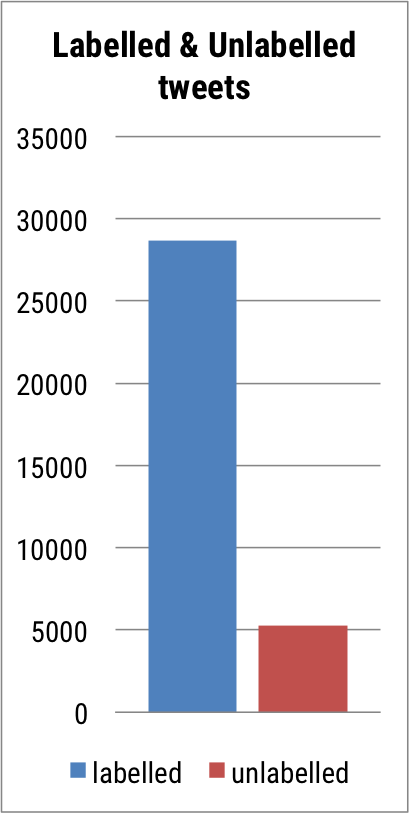
\includegraphics[width=0.3\textwidth]{EmotionLabel}
\caption{The result of emotion extraction from the dataset}
\label{fig:emotionLabel}
\end{figure}

\begin{figure}[!htb]
\centering 
\begin{subfigure}{0.5\textwidth}
\centering
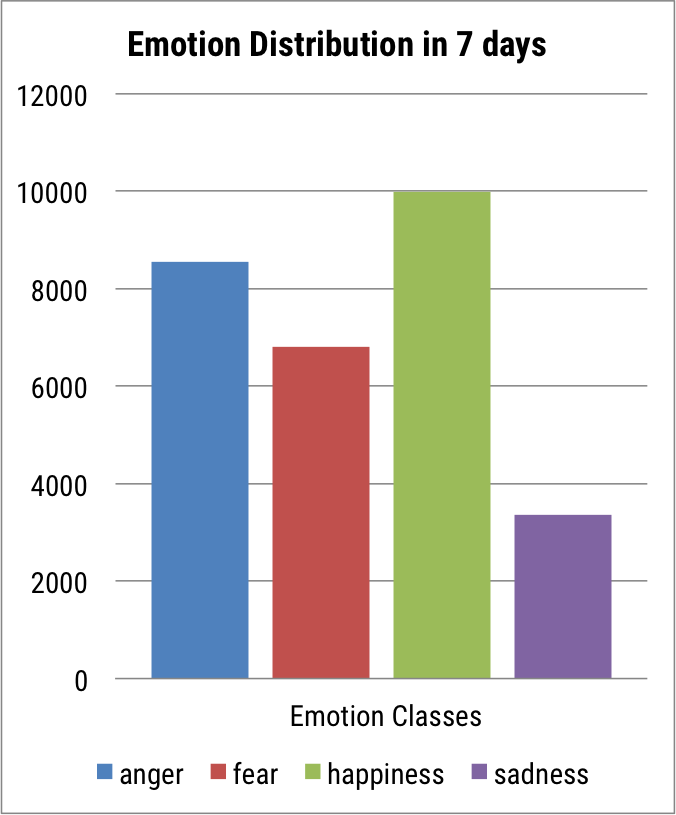
\includegraphics[width=0.75\linewidth]{EmotionDistributionWeek}
\caption{Seven days}
\label{fig:emotionDistributionWeek}
\end{subfigure}%
\begin{subfigure}{0.5\textwidth}
\centering
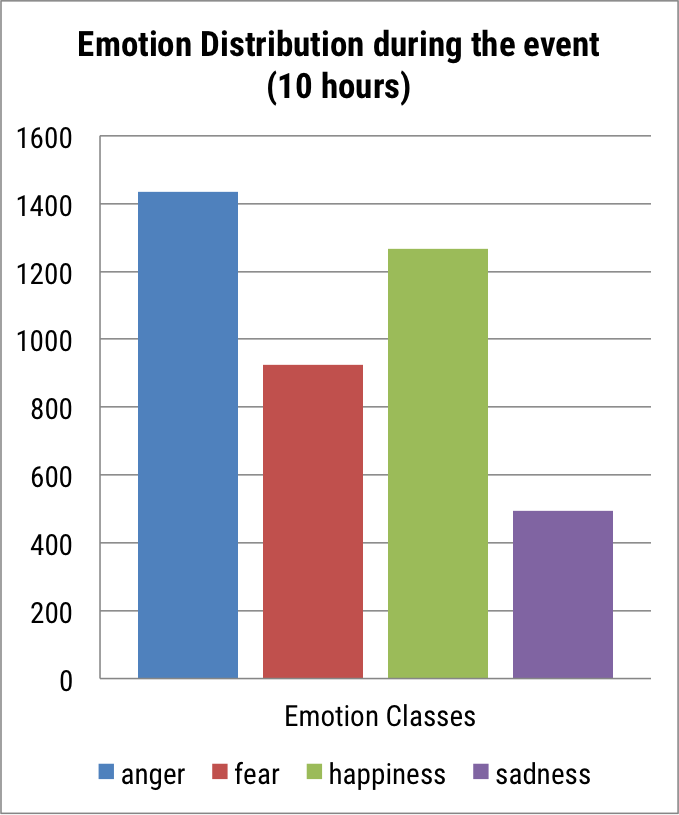
\includegraphics[width=0.75\linewidth]{EmotionDistributionEvent}
\caption{During event}
\label{fig:emotionDistributionEvent}
\end{subfigure}
\caption{The number of tweets labelled with each emotion in the whole dataset of seven days and during the event}
\end{figure}

Among the labelled tweets, the number of tweets in each emotion was not equally distributed as can be seen in Figure \ref{fig:emotionDistributionWeek}. This finding further supports the argument mentioned in Chapter \ref{ch:approach} that the users tend to post more happy content than the other emotions. 

The boxing match started at 6:00PM local time on May 3rd, while the stampede occurred around 10:45PM and the situation was reported to get under control at 1:00AM. There points were helpful to identify the time period that could be considered to be related to the event. The event was defined as a 7 hour period starting from 6:00PM to 1:00 AM. Our statistical analysis emphasised on this period. Figure \ref{fig:emotionDistributionEvent} illustrates the distribution of emotions during this event. As can be seen, the dominating emotion was \textit{anger}. The reason might be because of the nature of the boxing match that the related tweets contained lots of aggressive words.

\subsection{Statistical Analysis}

\subsubsection{Number of tweets labelled in each emotion over time}
Figure \ref{fig:emotionInstanceEvent} illustrates the change in the number of tweets labelled in each emotion over time. The horizontal axis presents our focused time-line consisting of 29 segments. The vertical axis shows the total number of tweets labelled with a specific emotion within a segment. The highlighted area between 10:45PM and 11:30PM illustrates the time when the stampede was reported to occur.

\begin{figure}[!htbp] 
\centering
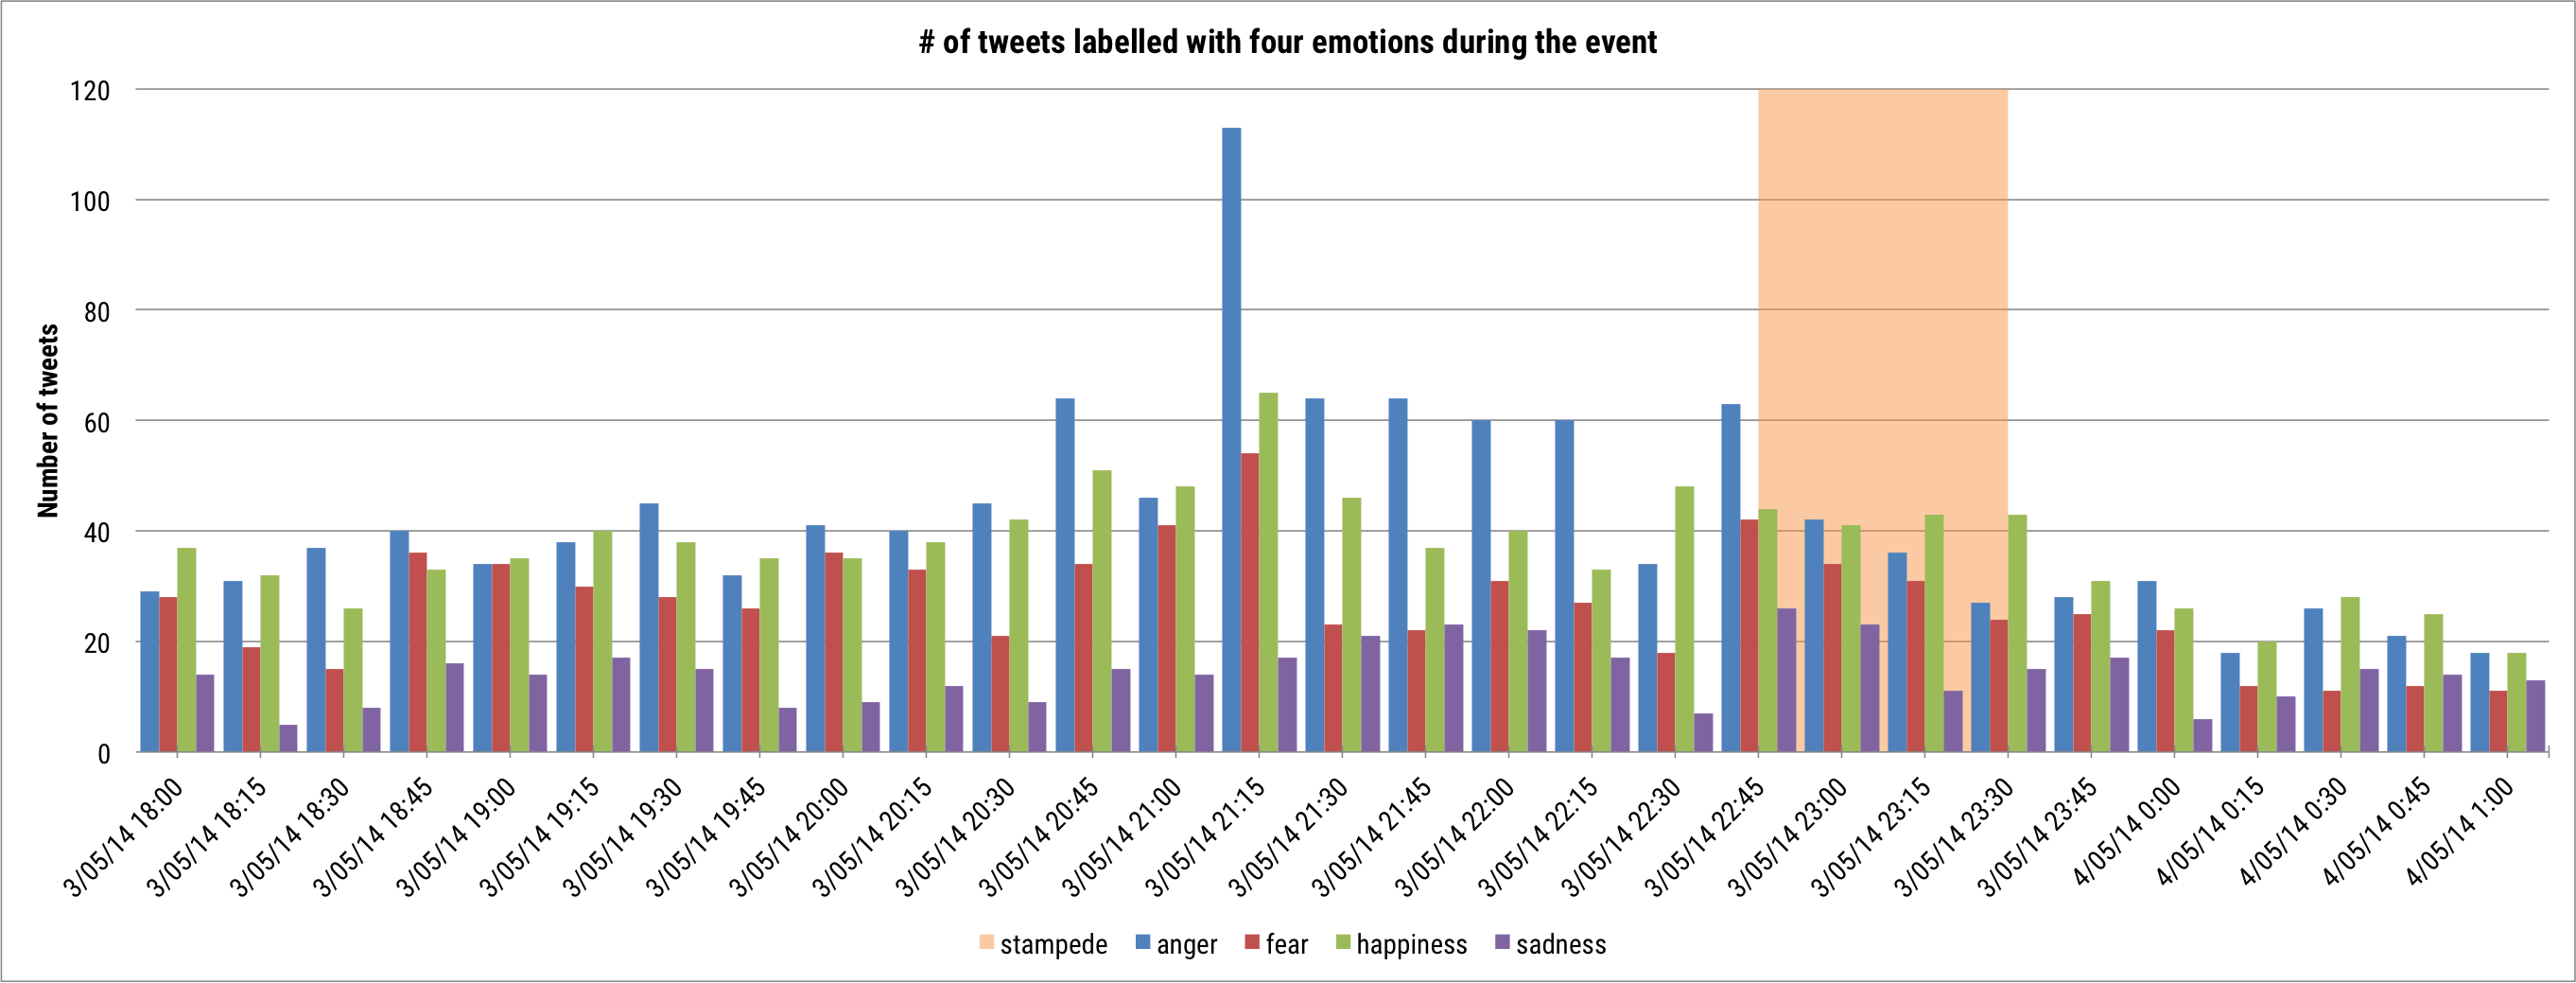
\includegraphics[width=1.0\linewidth]{EmotionInstanceEvent}
\caption{The number of tweets labelled with anger, fear, happiness and sadness during the event}
\label{fig:emotionInstanceEvent}
\end{figure}

As can be noticed from the charts, \textit{anger} labelled tweets reached a sudden peak at May 3rd 9:15PM. The number of tweets labelled with \textit{fear} and \textit{happiness} were also considerably high in this segment. Because of the overall increase trend across all emotions, the change caused by \text{anger} became less significant because there were increases in other emotions as well.

In conclusion, the number of tweets was not a robust measure to identify changes in emotion because it was affected by the overall trend. This also explained why emotion rate was selected as the measure in our approach.

\subsubsection{Emotion rate of each emotion over time}
Figure \ref{fig:emotionRateEvent} shows the emotion distribution over time using the emotion rate. 

\begin{figure}[!htbp] 
\centering
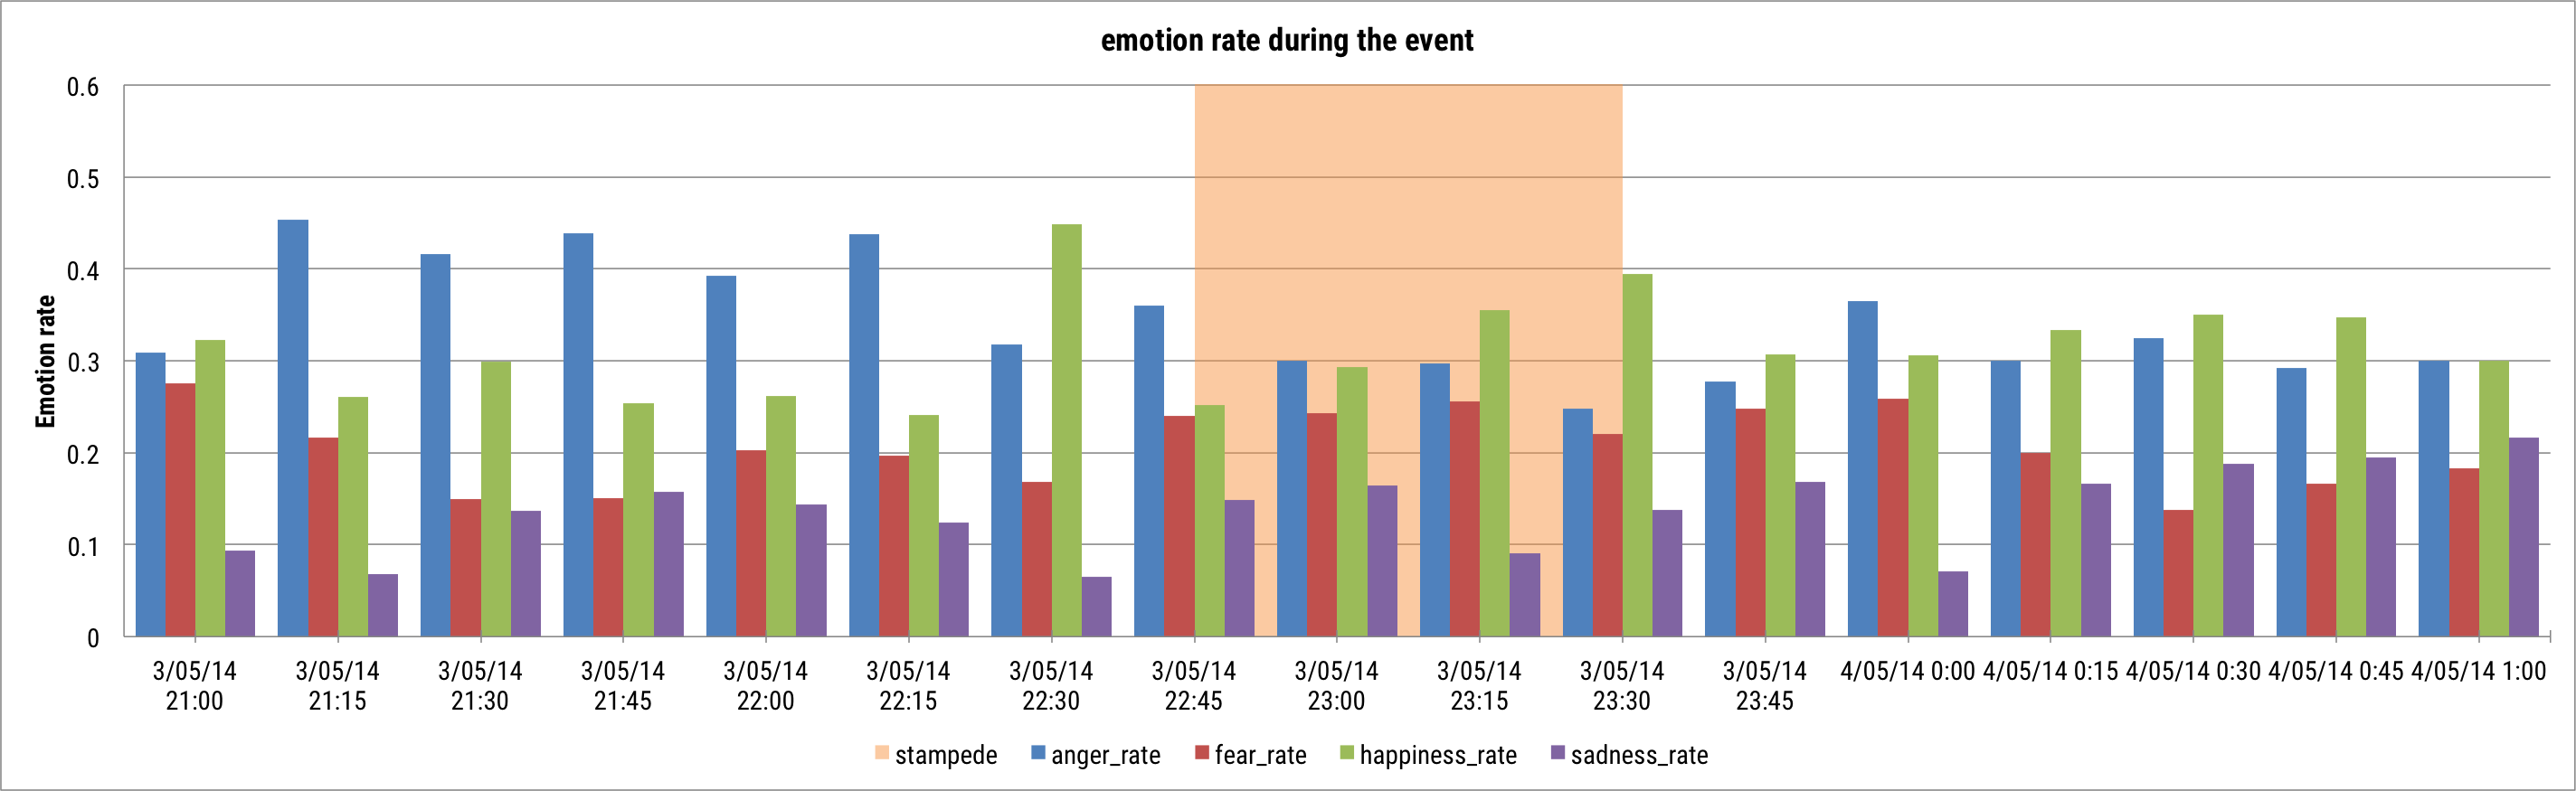
\includegraphics[width=1.0\linewidth]{EmotionRateEvent}
\caption{The percentage of anger, fear, happiness and sadness over time during the event}
\label{fig:emotionRateEvent}
\end{figure}

As can be seen, during the highlighted segments, \textit{happiness} was the emotion that had the highest rate among the four emotions. However, this rate started relatively high compared to other emotions at the beginning of the event period. Secondly, as mentioned earlier, the proportion of happiness labelled tweets was generally larger than other emotions during the seven days of sampling period. Therefore, a high value of the emotion rate can not be inferred to the behaviour of the crowd at a certain time. In fact, the changes of emotion rate over time was more important to identify abnormal behaviour in the crowd. This explained the use of moving average and z-score of emotion rate proposed in our implementation.

\subsubsection{The normal distribution of emotion rate over time}
This section investigates the distribution of emotion rate over time. By applying histogram to the emotion rate over time of each emotion, the distribution of the emotion rate followed the normal distribution. The majority of the values were close to the mean values forming a bell shape, as can be seen in Figure \ref{fig:histogramWeek}. In a normal distribution, the further a value deviates from the mean value, the less frequently it appears, thus suggesting a lower probability of occurrence. As mentioned earlier, the high level threshold was proposed as \(+1.0\). Because of the normal distribution, the probability of a high level emotion to occur is 15.8\%.

\begin{figure}[!h] 
\centering    
\begin{subfigure}{0.5\textwidth}
\centering
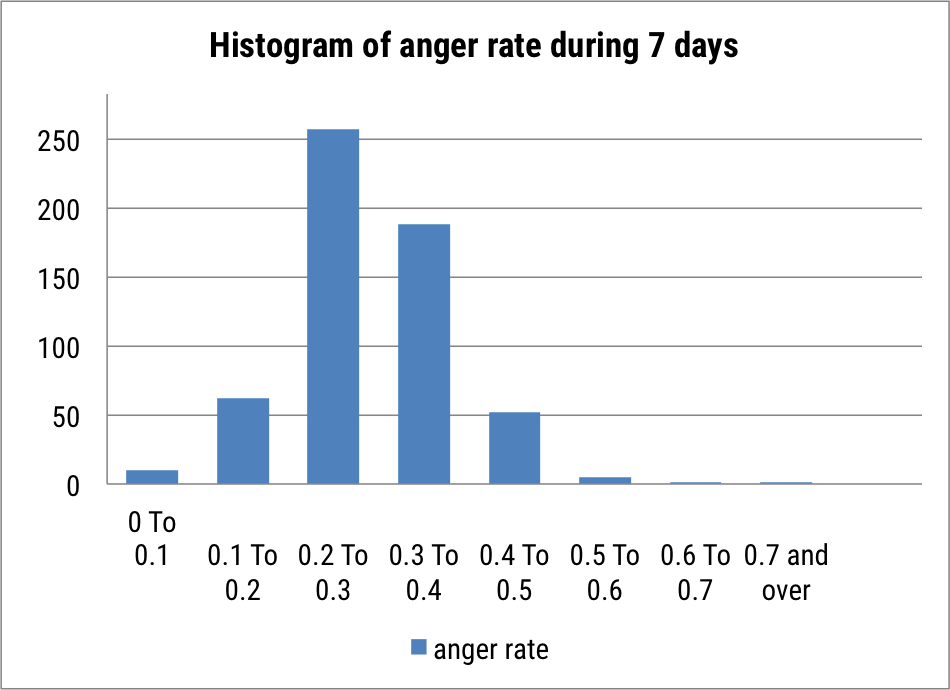
\includegraphics[width=0.98\linewidth]{HistogramAngerWeek}
\caption{anger}
\label{fig:histogramAngerWeek}
\end{subfigure}%
\begin{subfigure}{0.5\textwidth}
\centering    
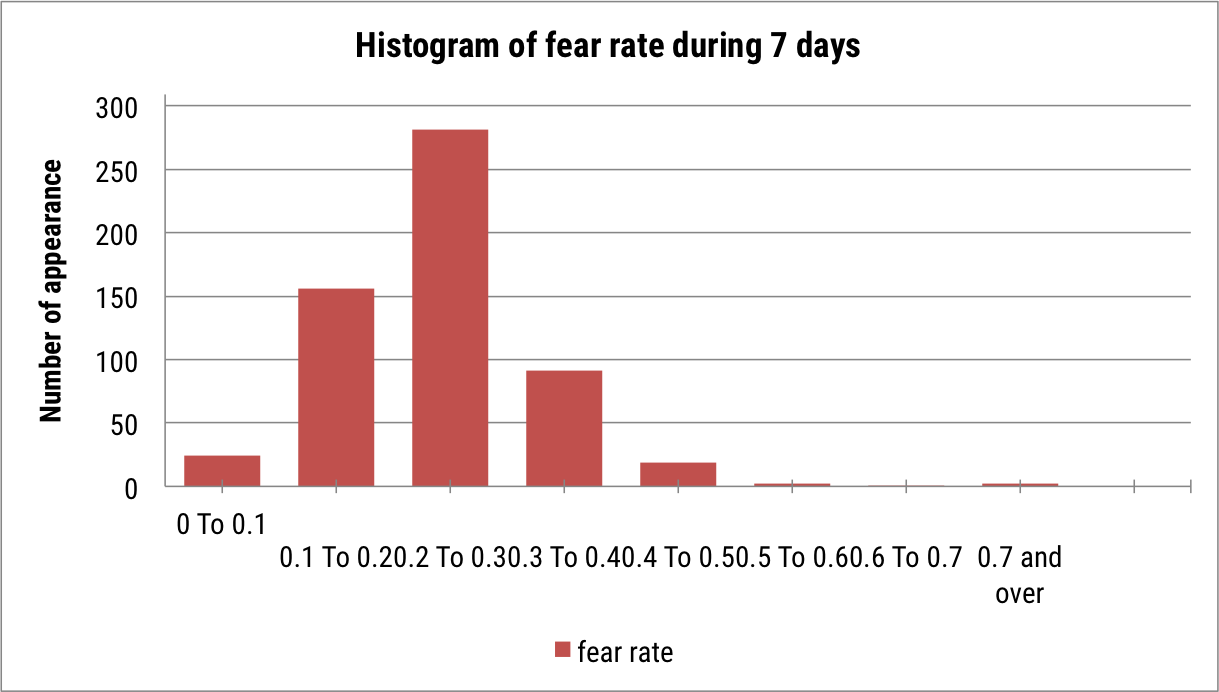
\includegraphics[width=0.98\linewidth]{HistogramFearWeek}
\caption{fear}
\label{fig:histogramFearWeek}

\end{subfigure}
\begin{subfigure}{0.5\textwidth}
\centering    
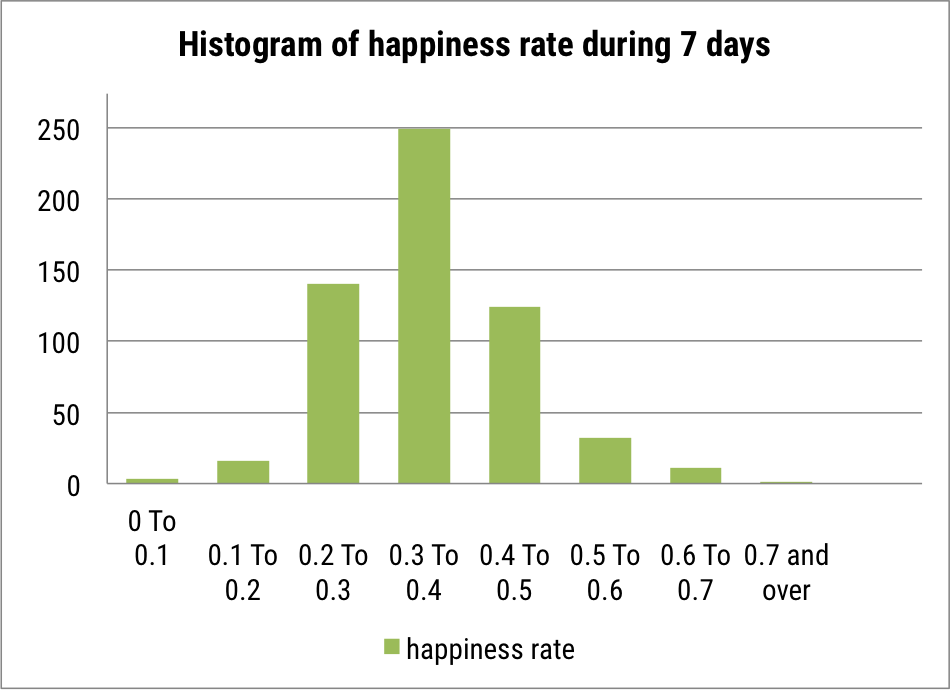
\includegraphics[width=0.98\linewidth]{HistogramHappinessWeek}
\caption{happiness}
\label{fig:histogramHappinessWeek}
\end{subfigure}%
\begin{subfigure}{0.5\textwidth}
\centering    
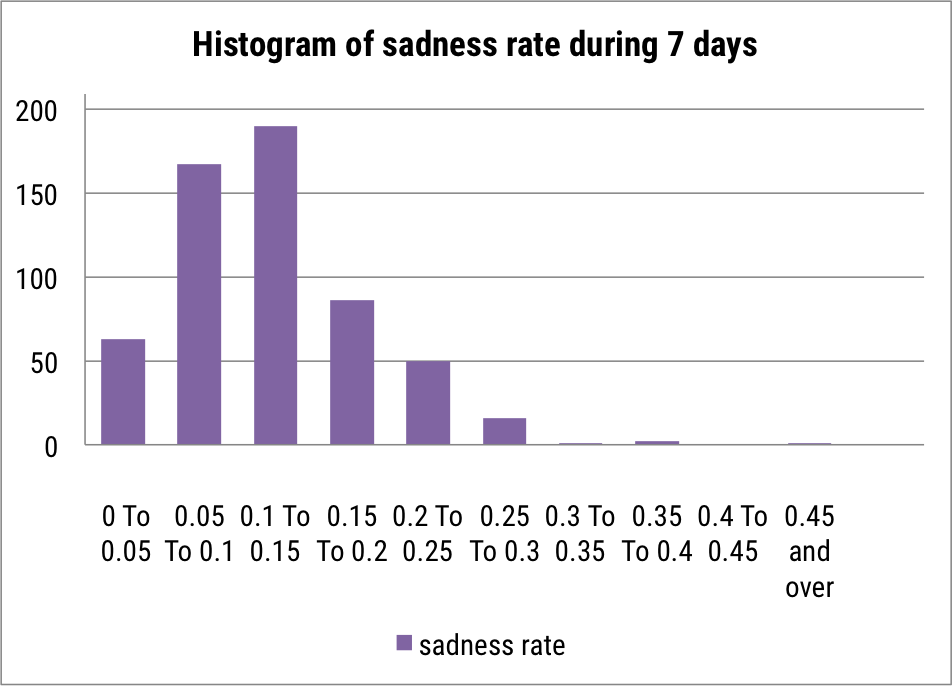
\includegraphics[width=0.98\linewidth]{HistogramSadnessWeek}
\caption{sadness}
\label{fig:histogramSadnessWeek}
\end{subfigure}
\caption{The normal distribution of anger, fear, happiness and sadness emotion rate over time in the dataset}
\label{fig:histogramWeek}
\end{figure}

\subsubsection{Z-score and the level of an emotion}
In statistics, z-score is a normalized score representing whether an observed value is lower or higher than the mean value and how far the deviation is. In our experiment, z-score was effective when combined with moving average to detect changes in emotion rate. Figure \ref{fig:emotionZscoreEvent} presents the z-score of emotion rate of the four emotions over time during the event. As can be seen, at 10:45PM when the stampede was reported to start, the z-scores of \textit{anger} and \textit{happiness} emotion rate were negative, suggesting that their emotion rates were below the expected value. On the other hand, the z-scores of \textit{fear} and \textit{sadness} emotion rate were positive. 

\begin{figure}[!htb] 
\centering
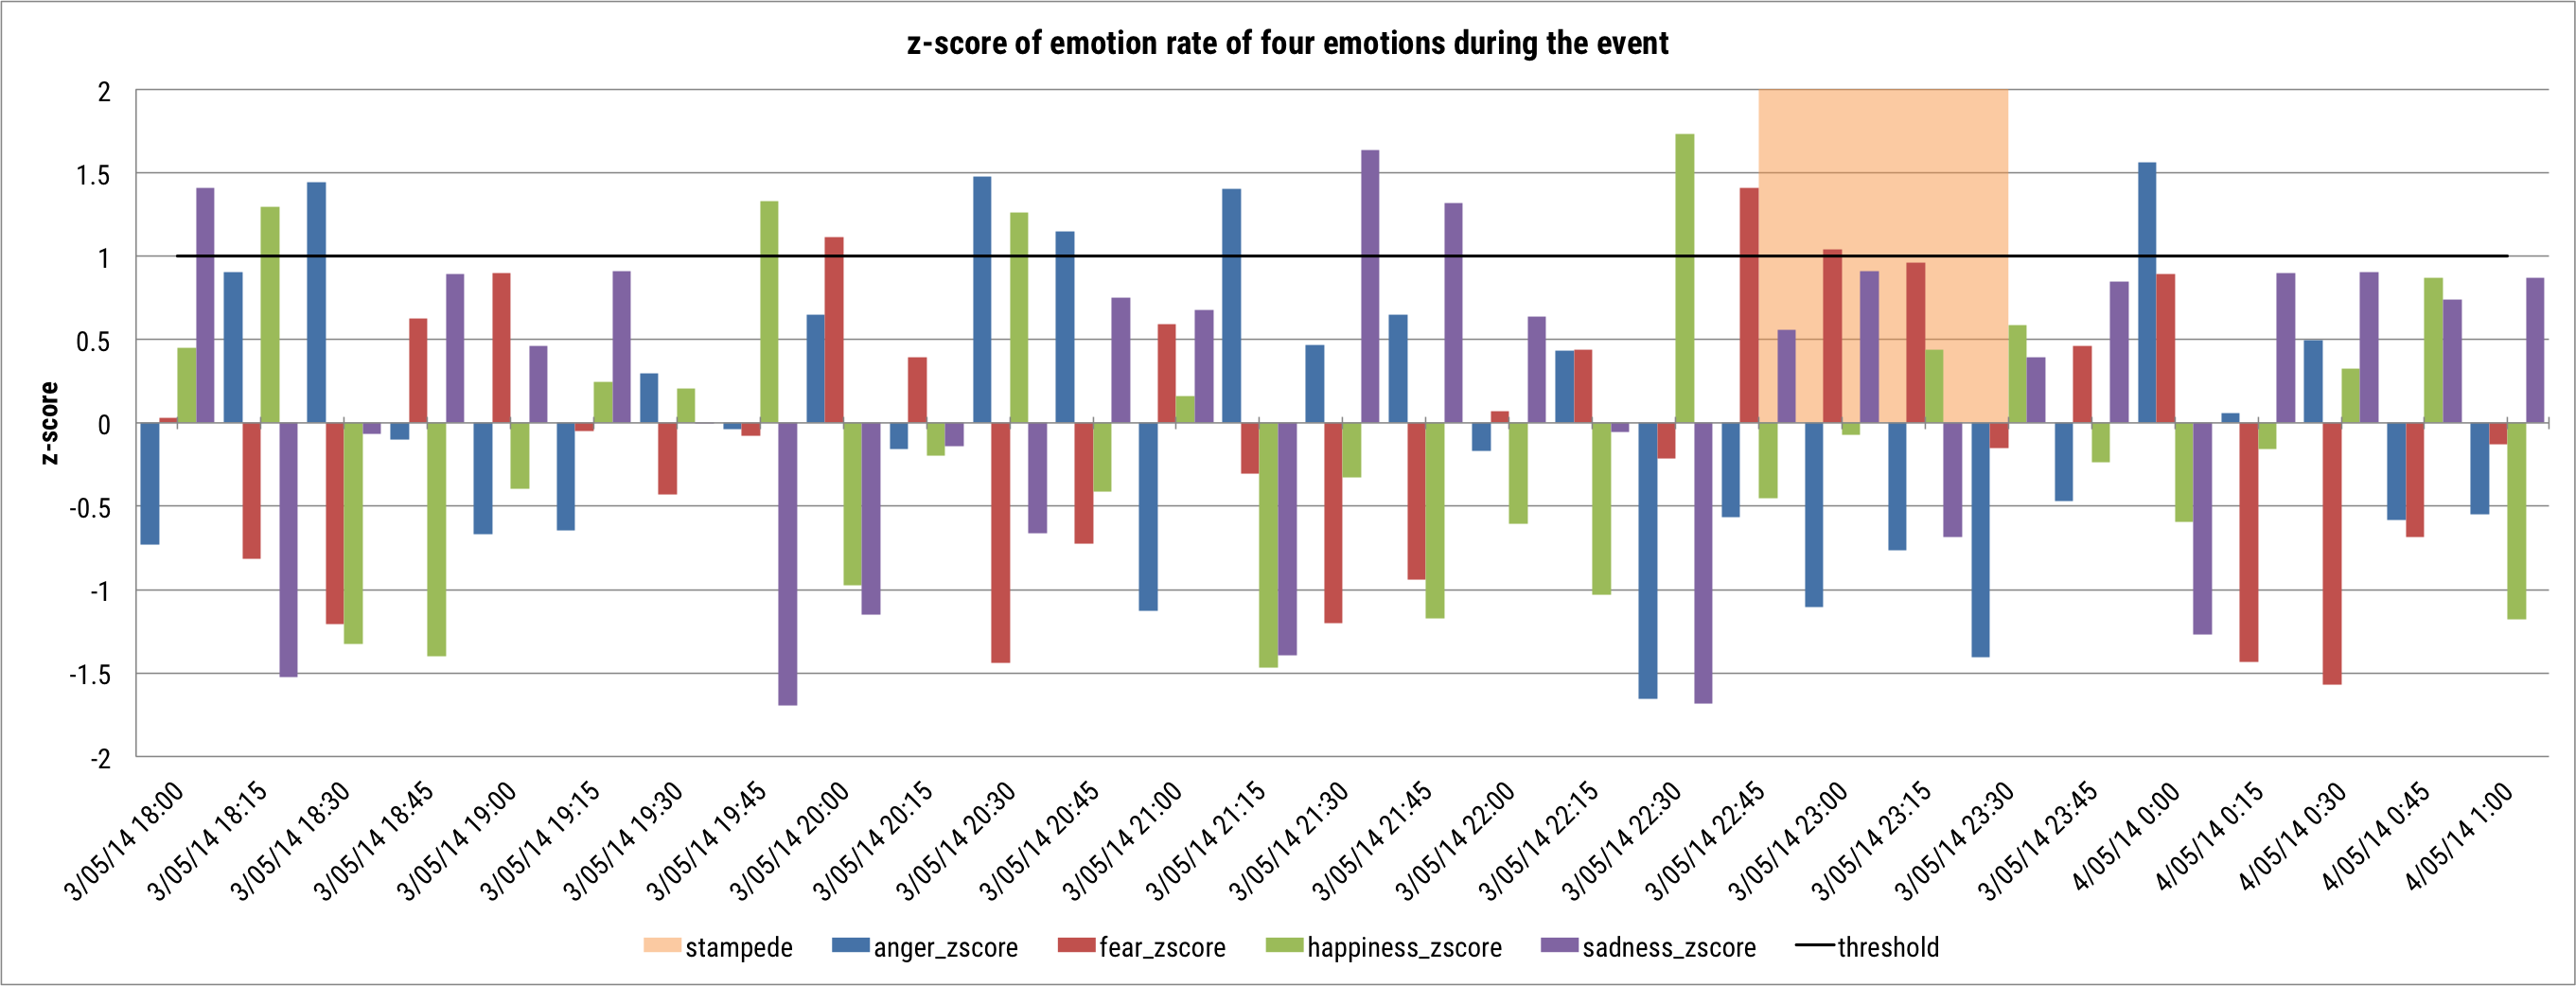
\includegraphics[width=1.0\linewidth]{EmotionZscoreEvent}
\caption{The z-score of anger, fear, happiness and sadness rate over time during the event}
\label{fig:emotionZscoreEvent}
\end{figure}

\begin{figure}[!htb]
\centering
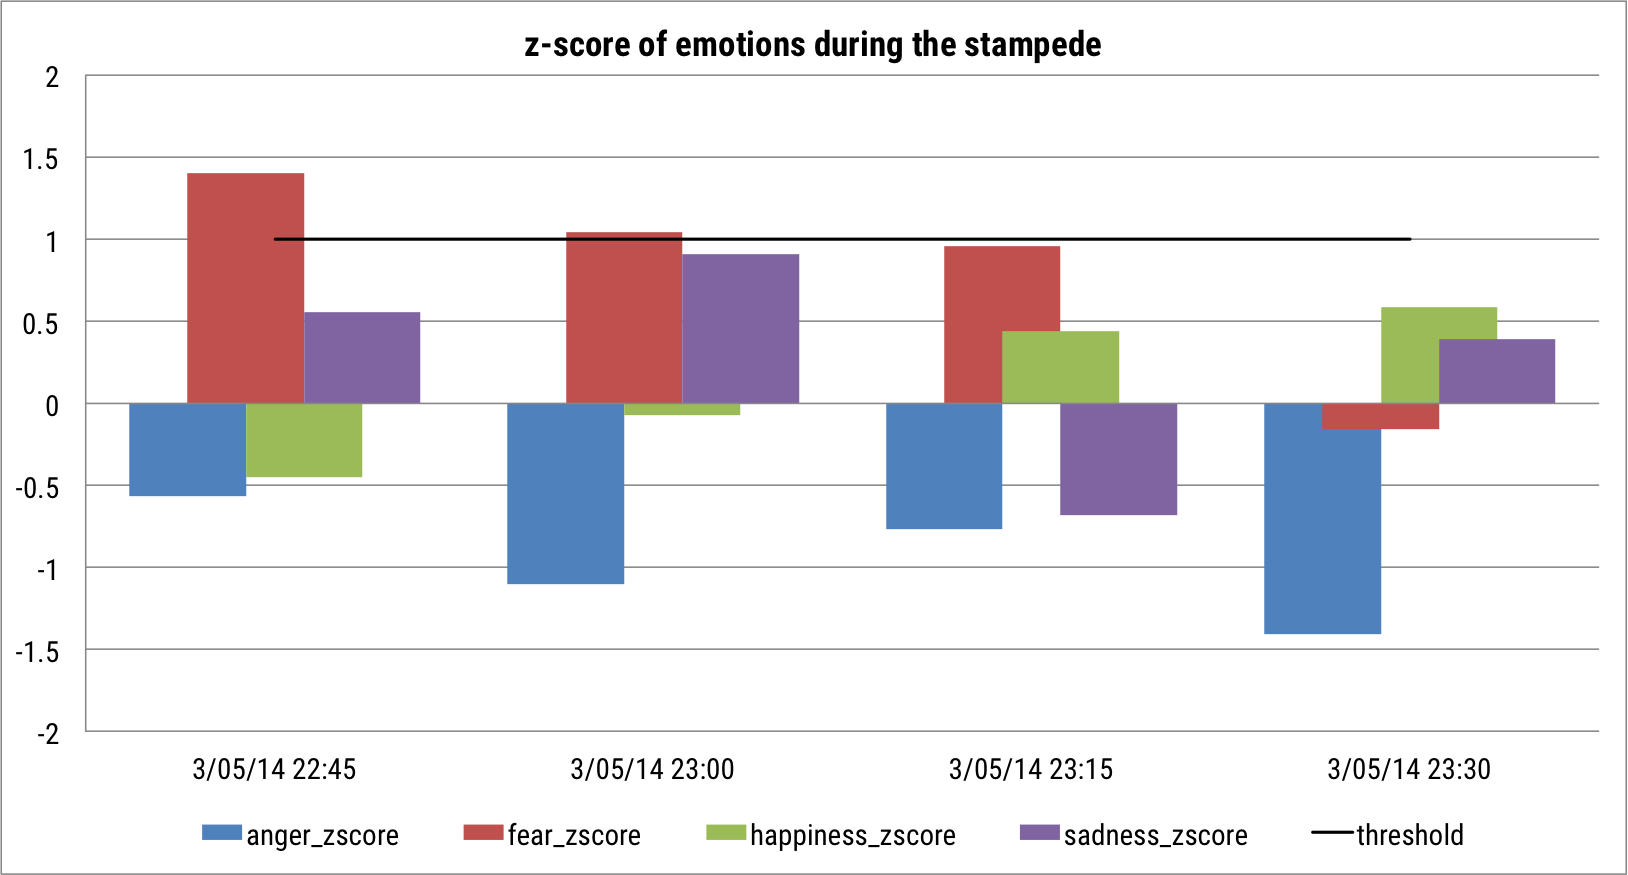
\includegraphics[width=1.0\textwidth]{EmotionZscoreFocus}
\caption{Threshold and z-score of emotions}
\label{fig:emotionZscoreFocus}
\end{figure}

Figure \ref{fig:emotionZscoreFocus} focuses on the one hour period when the stampede was happening. The threshold line represents our chosen high level threshold. It was noticeable that among four emotions, only \textit{fear} exceeded this threshold in two segments at 10:45PM and 11:00PM. It showed that when the stampede occurred there was a significant increase in the proportion of tweets labelled with \textit{fear}, suggesting a high level of fear in the crowd.

\subsubsection{Crowd Types Reasoning}
Figure \ref{fig:crowdTypeStampede} shows the result of the Rule Based Reasoning based on the levels of emotions. As can be seen, the inferred crowd types when the stampede occurred at 10:45PM stood out as the escaping crowd and the dense/suffocating crowd. These crowd types belong to Group 4 which is motivated by fear.

\begin{figure}[!htbp]
\centering
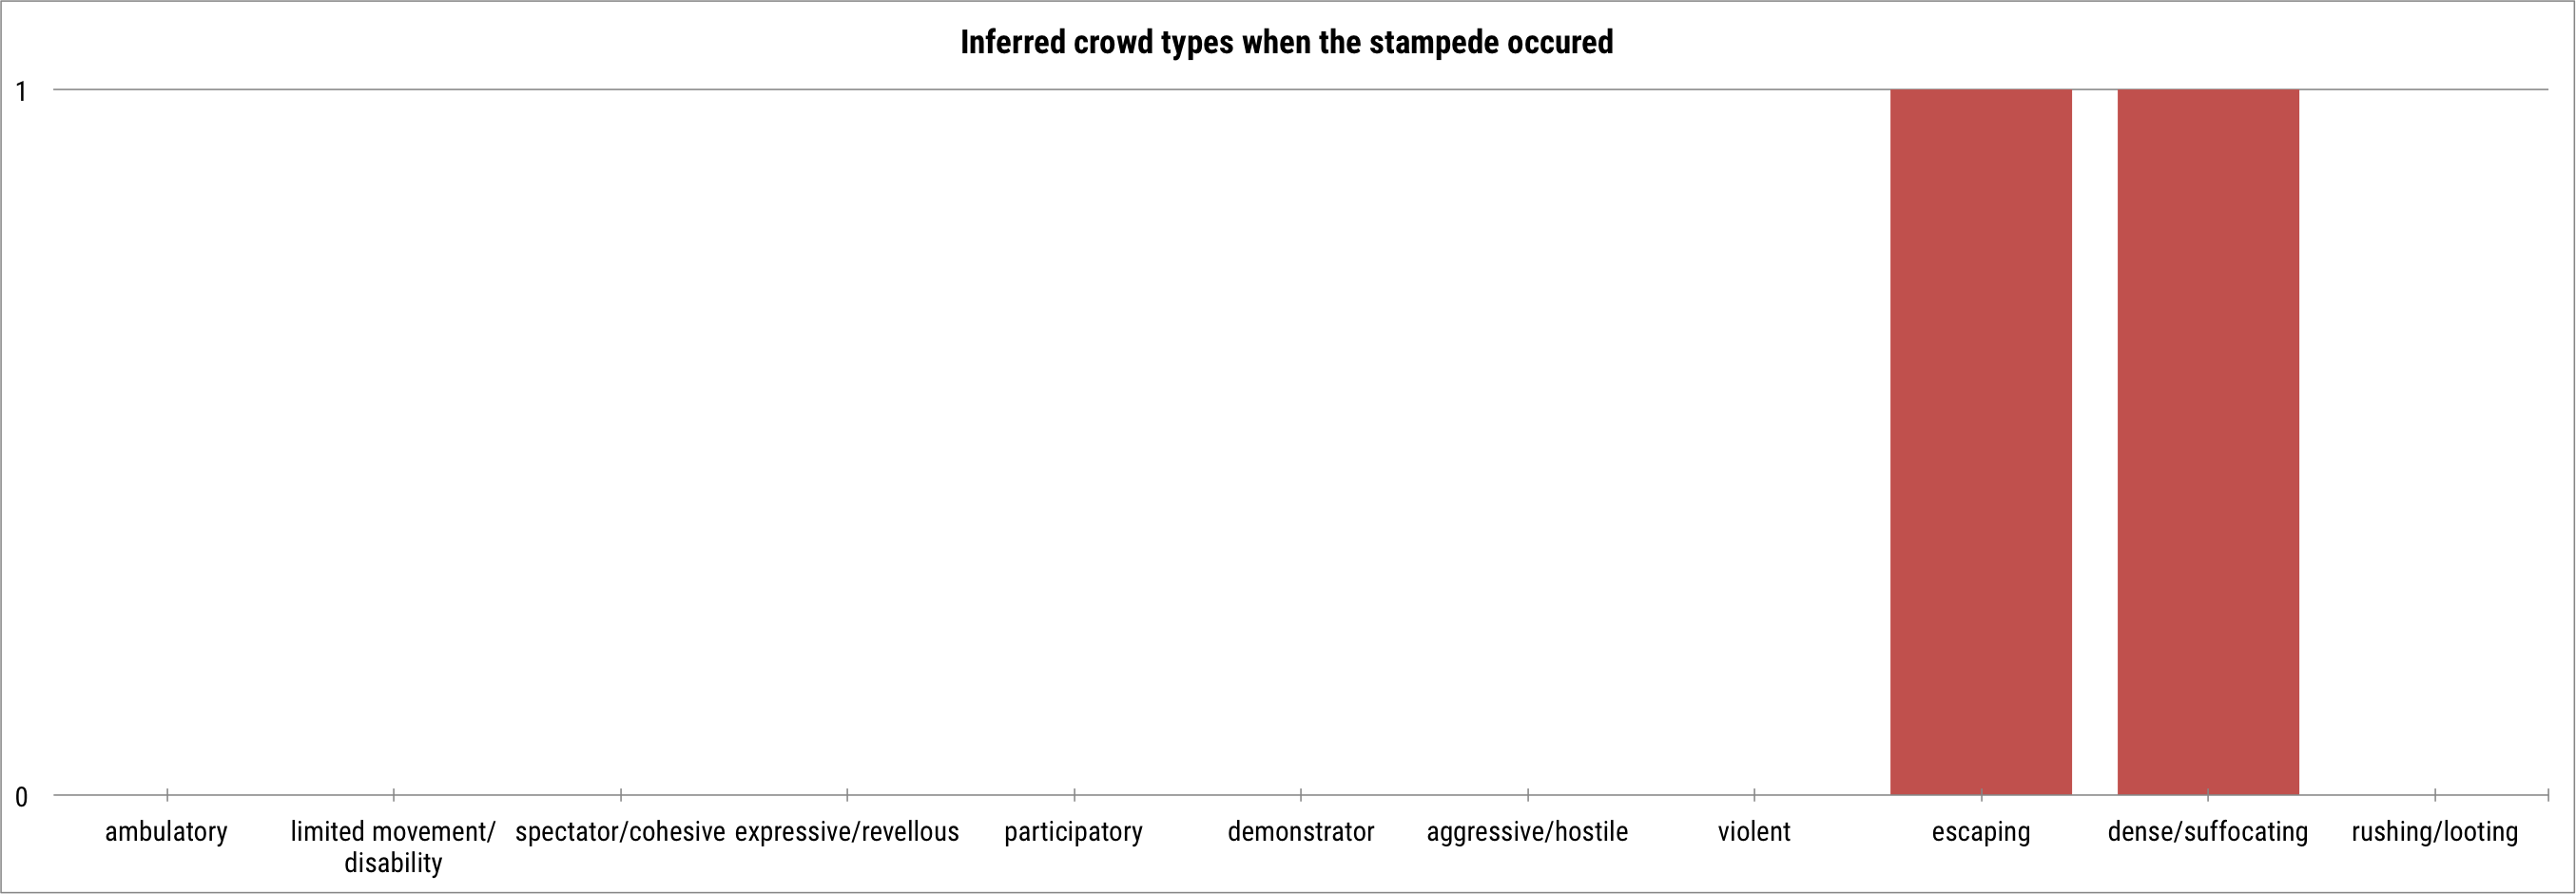
\includegraphics[width=0.75\textwidth]{CrowdTypeStampede}
\caption{Inferred crowd types where the stampede occurred}
\label{fig:crowdTypeStampede}
\end{figure}

\subsection{Discussion}

\subsubsection{Correctness and Timeliness of the Detection}
Firstly, regarding correctness of the detection, the inferred crowd types matched with the reported crowd types occurred the incident that were escaping and dense/suffocating crowd. Although our defined rules only lead to the group of crowd types rather than the exact crowd types, in this case study the rules were sufficient to point out a dangerous situation in the crowd.

In term of timeliness, using our proposed Emotion Analysis of the social media, the escaping crowd and dense/suffocating crowd were detected in the 10:45PM segment. It suggests that in a real-time monitoring, the result can be obtained the soonest at 11:00PM if the interval is selected as 15 minutes as in the experiment. According the official announcement, the local police received a phone call reporting about the stampede at 10:45PM, which was relatively close to our time of detection.

The case study has confirmed the capability of our proposed framework in term of producing correct and timely detection as soon as the stampede occurred. The collected data also brings forward questions and potential future researches which will be discussed in following sections.

\subsubsection{The shift in emotion during the event}
As mentioned earlier, tweets labelled with \textit{happiness} dominated the emotion distribution in the large sampling period of seven days. However, focusing on the data collected during the event, the number of tweets labelled with \textit{anger} surpassed that of \textit{happiness}. The reason for this shift in emotion might be due to the nature of the event which was a boxing match. The tweets related to a boxing match might contain words that associate to a certain degree of aggressiveness. This leads to the next question that whether the type of event has significant effect on the emotions of the people in the crowd or not, which will require further study.

\subsubsection{Behaviour in an emergency situation}
Another interesting discovery by further investigating collected data is context of tweets mentioning about the stampede when they were posted. It can be noticed that a large number of those tweets were not posted from the crowd. The first scenario is that the tweet was posted after the user safely got out of the crowd. It appears to be reasonable that during such an emergency situation, people would prioritise escaping over posting about it on social media. The second scenario is that the author of the tweet was not participating in the event and only reported about the incident. In this scenario, the author might be or not be influenced by the same emotion as the people in the crowd. Therefore, future researches are required to investigate further on the behaviour of people under emergency situation and the effect of emotion on people outside the crowd.

Table \ref{table:tweetStampede} extracts some tweets containing keyword ``stampede'' posted around the time of the incident. Most tweets seems to be posted under first scenario, while the last tweet belongs to the second scenario. Nevertheless in our research, both scenarios were able to offer information about the occurrence of the stampede, which was useful for our analysis to detect the emergency situation.

\begin{table}[!htb]
\centering
\caption{Sample tweets mentioning about the stampede}
\label{table:tweetStampede}
\begin{tabular}{|p{3cm}|p{12cm}|}

\hline
\textbf{Posted time} & \textbf{Tweet} \\ \hline \hline
2014-05-03 22:49:16 & A stampede of people just rushed into the media room a was very hectic Here at the MGM Grand \#TheMoment \#boxing \#boxeo \\ \hline
2014-05-03 22:53:00 & Was nearly trampled during a frightening stampede leaving MGM Grand Garden. Not the highlight of this trip. \#TheMoment \\ \hline
2014-05-03 23:15:05 & Crazy scenes @MGMGrand as shots were fired, we were caught in the stampede following the @floydmayweather flight. Many people injured. \\ \hline
2014-05-03 23:16:05 & Scary scenes at the MGM grand after the Mayweather fight apparently a gun was shot which caused a stampede plp crushed scary shit \\ \hline
2014-05-03 23:29:58 & Crazy fight, crazy night. Almost got trampled in a stampede outside the arena. Fights breaking out everywhere. Ugly atmosphere. \\ \hline
2014-05-03 23:57:46 & My friend just left the \#MayweatherMaidana fight @MGMGrand \& called to tell me she was scared but safe. \#stampede? \\ \hline
\end{tabular}
\end{table}

\subsubsection{Potential of Prediction}
Although crowd monitoring operation does not involve forecasting, the capability to predict an emergency situation will benefit the emergency management in the perspective of planning and preparation. Comparing the emotion rates of \textit{anger}, \textit{fear}, \textit{happiness} and \textit{sadness} before and after the occurrence of the stampede, an interesting pattern of change in emotion can be noticed. Figure \ref{fig:emotionRatePrediction} illustrates the emotion rate of the four emotions in two segments before and after the stampede occurred respectively. As can be seen, the emotion rate of \textit{happiness} dropped remarkably while the rates of the other three emotions rose. Because \textit{happiness} can be considered as a positive emotional state whereas \textit{anger}, \textit{fear} and \textit{sadness} have the negative tendency, this change in emotion might suggest a possible emergency situation.

\begin{figure}[!htbp]
\centering
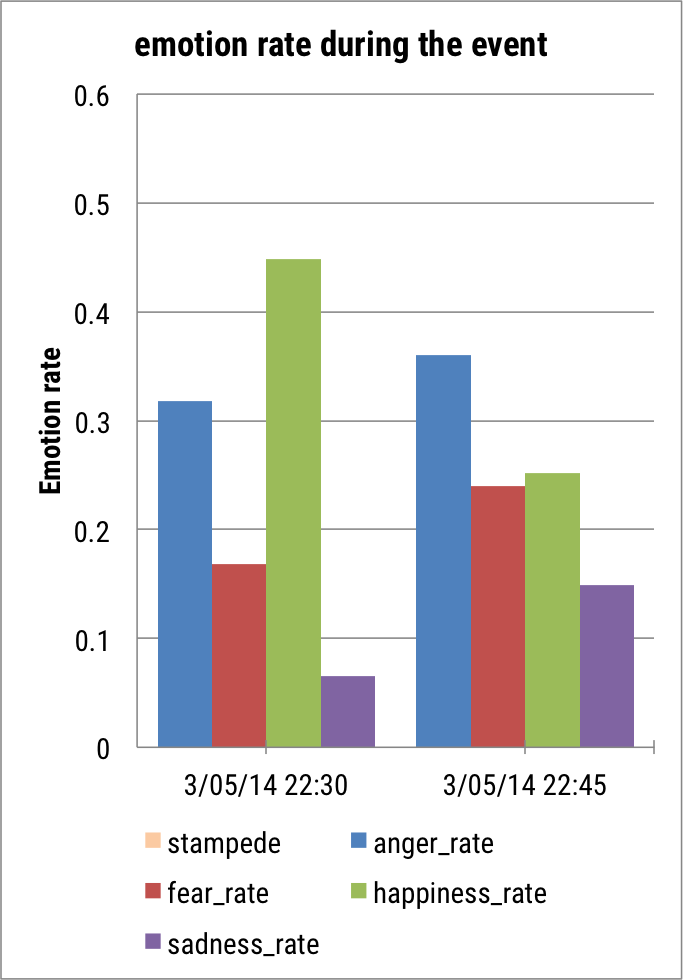
\includegraphics[width=0.4\textwidth]{EmotionRatePrediction}
\caption{Emotion rates of the four emotions before and after the occurrence of the stampede}
\label{fig:emotionRatePrediction}
\end{figure}

\section{Conclusion}
This chapter has described our evaluation of the proposed Crowd Monitoring Framework using a stampede accident occurred in a selected sporting event as a case study. A simple implementation to illustrate the framework's process has been introduced with moving average and z-score as the factors to determine the threshold for the high level of an emotion. The result of the experiment shows that using Emotion Analysis on the tweets collected about the event, the correct crowd types can be identified in a timely manner.